\documentclass[10pt,a4paper,twoside, french]{article}
\addtolength{\textheight}{90pt} \addtolength{\topmargin}{-60pt}
\textwidth 164mm \oddsidemargin -2mm \evensidemargin -2mm
\usepackage[utf8]{inputenc}
\usepackage[T1]{fontenc}
\usepackage[english]{babel}
\usepackage{enumerate}
\usepackage{graphicx} 
\usepackage[left=2.5cm,right=2.5cm,top=3.5cm,bottom=3.5cm]{geometry}
%\usepackage{xcolor,rotating,epic,eepic}
\usepackage[font=small,labelfont=bf]{caption}  %% titre dans les minipage
\usepackage{subcaption} %% les sous figure pour les sous legendes
\usepackage{mathtools}   %%   package mathematique
\usepackage{amssymb}  %% symbole mathematique
\usepackage{fancyhdr}  %% pour pied de page et entete et layout
\usepackage{fourier}  %%  police
\usepackage{titlesec}  %% modifier les section
\usepackage{pgfplots} %% provides tools to generate plots and labeled axes easily
\usepackage{color}

\usepackage{tikz}  %%pour les figures
\usetikzlibrary{positioning}
\usepgfplotslibrary{external}
\tikzsetexternalprefix{External-TikZ/}
\tikzexternalize
\tikzset{math3d/.style=
    {y= {(0.353cm,0.353cm)}, z={(0cm,1cm)},x={(1cm,0cm)}}}
\usepackage[colorlinks = true,
            linkcolor = blue,
            urlcolor  = blue,
            citecolor = black,
            anchorcolor = blue]{hyperref} %% permet de renvoyer à la section en cliquant sur la table des matieres
            
            
            
%ecriture des algo
\usepackage{listings}
\lstset{
	language= Matlab,  %choix du language
    frame=tb, % tb=draw a frame at the top and bottom  - single=around
    tabsize=4, % tab space width
    breaklines=true,
    showstringspaces=false, % don't mark spaces in strings
    backgroundcolor=\color{gray!10},
    numbers=none, % display line numbers on the left
%    numbersep=10pt,                   % how far the line-numbers are from the code
%    numberstyle=\normal\color{black}, % the style that is used for the line-numbers
    commentstyle=\color{red}, % comment color
    keywordstyle=\color{blue}, % keyword color
    stringstyle=\color{green}, % string color
    xleftmargin=17pt,
    framexleftmargin=17pt,
    framexrightmargin=0pt,
    framexbottommargin=5pt,
    framextopmargin=5pt,
    escapeinside={(*}{*)}
}
\DeclareCaptionFormat{listing}{\hrulefill\par\vskip1pt#1#2#3}
\captionsetup[lstlisting]{format=listing,singlelinecheck=false, margin=0pt, font={sf},labelfont=bf}
%font={sf}  labelsep=space   %option captionsetup, ,\rule{\dimexpr\textwidth\relax}{0.4pt}

\renewcommand\lstlistingname{Algorithm}  % CHANGER NOM LISTING EN ALGORITHM
%%%%%%%%  Style subsection  %%%%%%%%%%
\usepackage{titlesec}  %% modifier les section
\titleformat*{\section}{\bf}
\titleformat*{\subsection}{\rm}

\numberwithin{equation}{section}
\numberwithin{figure}{section}
\numberwithin{table}{section}

%%%%%%%%%%%  COMMANDE  %%%%%%%%%%%%%%%%%%%%%%%
\newcommand{\vect}[1]{\mathbf{#1}}
\newcommand{\eq}{\Longleftrightarrow}
\newcommand{\chap}[1]{\widehat{#1}}
\newcommand{\R}{\mathbb{R}}
\newcommand{\N}{\mathbb{N}}
\newcommand{\Po}{\mathbb{P}}
\newcommand{\EspAp}[1]{\text{\textbf{#1}}_h}
\newcommand{\enstq}[2]{\left\{#1\mathrel{}\middle|\mathrel{}#2\right\}}
\newcommand{\nm}{|\!|\!|}
\newcommand{\norme}[1]{\left\Vert #1\right\Vert}
\renewcommand{\div}[1]{\text{div } \vect{#1}}
\newcommand{\rot}[1]{\text{\textbf{rot} } \vect{#1}}
\newcommand{\grad}[1]{\text{\textbf{grad} } \vect{#1}}
\newcommand{\diff}{\mathop{ }\mathopen{ }\mathrm{d}}
\newcommand{\restreinta}[1]{\mathclose{}|\mathopen{}_{#1}}
\newcommand{\prodscal}[2]{\left( #1\ ,\ #2\right)}


\begin{document}

\begin{figure}[h]
\centering

\includegraphics[scale=.5]{fig/kth}
\vspace{-1.5cm}
\end{figure}
	\vspace{1cm}    
    \begin{center}
       		\rule{10cm}{1pt} \\[0.6cm]         %% ligne horizontale   \rule[raise-height]{width}{thickness}  
        	{\huge Homework Assignment 2 \\[0.2cm]
         \Large  Numerical analysis for PDE's\\[0.2cm] 
          \large Thomas Frachson - Davoud Saffar Shamshirgar}  \\[0.6cm]
    		\rule{10cm}{1pt} \\[0.5cm]  
	\end{center}    
	
\setcounter{section}{1}
\begin{enumerate}
\item
\item
\item \begin{enumerate}[a.]
\item Considering the the following second order PDE
\begin{align*}
\mathfrak{L} = -(u_{xx}+2u_{xy}+u_{yy})=0,
\end{align*}
and the following schemes
\begin{align}
\mathfrak{L}_{\Delta_1}=\dfrac{1}{h^2}&(2u_{i+1,j}+2u_{i,j+1}+2u_{i-1,j}+2u_{i,j-1}-6u_{i,j}-u_{i+1,j-1}-u_{i-1,j+1}),\\
\mathfrak{L}_{\Delta_2}=\dfrac{1}{h^2}&(u_{i+1,j+1}-2u_{i,j}-u_{i-1,j-1}),
\end{align}
we can show that the schemes above are consistent. Note that the schemes have the following stencils.
\begin{figure}[h]
\centering
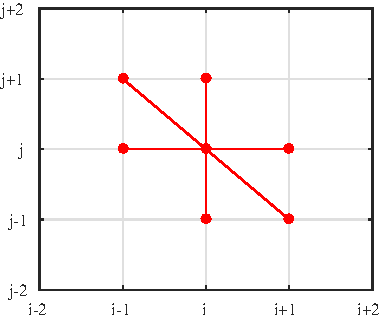
\includegraphics[scale=.8]{fig/scheme1}
\hspace{.8cm}
\includegraphics[scale=.8]{fig/scheme2}
\caption{Stencil for the scheme 1 (left) and scheme 2 (right).}
\end{figure}
To show that these schemes are both consistent, we start by doing a Taylor expansion.
\begin{align}
u(x+ih,y+jh) = u(x,y) +h(iu_x+ju_y)+\dfrac{h^2}{2}(i^2u_{xx}+iju_{xy}+j^2u_{yy})+{\cal{O}}(h^3).
\label{eq:taylor}
\end{align}
Using equation \eqref{eq:taylor}, we can write the schemes above as
\begin{align}
\mathfrak{L}_{\Delta_1}-\mathfrak{L} =  C_1h^2 + \mathcal{O}(h^3),\\
\mathfrak{L}_{\Delta_2}-\mathfrak{L} =  C_2h^2 + \mathcal{O}(h^3).
\end{align}
From this, it is easy to verify that 
\begin{align*}
\lim_{h\to0}\mathfrak{L}_{\Delta_i}-\mathfrak{L} = 0, \quad i=1,2.
\end{align*}
This proves the consistency of both methods.

\end{enumerate}


\end{enumerate}
	
	
	
	
\end{document}	
